% Figure 1: system architecture.
% Hand-specified diagram, no data input. Sources checked:
%  - actors, agents and wallet: the manuscript, Section "System Overview and Actors" and the application scenario;
%  - holder binding: the manuscript ("presents the credential itself to a Verifier, without a verifiable presentation");
%  - node or RPC provider: the manuscript, Section "Trust Assumptions" (trusted for the integrity and availability of its
%    replies; sees which identifiers are queried) and "Verifiers still read it through an RPC provider or their own node";
%  - controller functions and pause scope: contracts/DIDRegistry.sol (createDID 261-266 whenNotPaused;
%    updateDID 300-308, reactivateDID 343-347, changeController 365-371, acceptController 390-394, rotateKey 445-452,
%    addDelegate 610-616, removeDelegate 635-640, setAttribute 683-688: whenNotPaused; deactivateDID 327-330,
%    cancelControllerChange 420-423, revokeCredential 542-548: not paused, onlyController; repeated revocation
%    reverts 551-554; pause/unpause 728-733 and addAdmin/removeAdmin 713-718: onlyAdmin);
%    the controller list in the Issuer note is an example list ("for example"), not the full set;
%  - verifier reads: src/vc/verifier-service.js 152-224 (B0 block number; verifyDID twice,
%    getDIDDocument, isCredentialRevoked, all at that block); the checks are V1 to V7 and V8 accepts (Figure 2);
%  - subject DID registered by its own controller: scripts/measure-local.js 83-84;
%  - administrator powers and limits: the manuscript, Section "Registry Administration and Decentralisation"
%    ("The administrator role gives no power to change keys, documents or revocation records."); pause and unpause
%    are transactions, so the Administrator arrow also breaks at a stub of the node strip;
%  - DID record fields: the manuscript, Section 4.3, and the contract struct, including the nonce.
% Encoding shared with Figures 2 and 3: DID records sky #56B4E9 tint with a #2E86B8
% line; revocation records vermilion #D55E00 tint with a #D55E00 line; solid arrow = data transfer or transaction;
% dashed arrow = read-only query that sends no transaction; layer labels and secondary structure in grey #595959.
% Built at its printed width: the manuscript includes it at \columnwidth = 504.50787 pt (Times1COL), scale 1.0.
% Fonts: Times (mathptmx) and Courier (pcr), as in the manuscript. Smallest text 7 pt.
% Build: see build_all.sh (pdflatex gen_fig_1.tex, output copied to Figure_1.pdf).
\documentclass[border=0pt]{standalone}
\usepackage[T1]{fontenc}
\usepackage{mathptmx}
\renewcommand{\ttdefault}{pcr}
\usepackage[protrusion=false,expansion=false]{microtype}
\usepackage{tikz}
\usetikzlibrary{arrows.meta}
\pdfinfoomitdate=1 \pdftrailerid{} \pdfsuppressptexinfo=-1

% Okabe-Ito colours and the shared greys
\definecolor{oiverm}{HTML}{D55E00}
\definecolor{oisky}{HTML}{56B4E9}
\definecolor{skyline}{HTML}{2E86B8}
\definecolor{greytext}{HTML}{595959}
\definecolor{greyline}{HTML}{7F7F7F}
\definecolor{nodefill}{HTML}{EFEFEF}
\definecolor{regfill}{HTML}{F4F4F4}

\newcommand{\fn}[1]{{\fontsize{7}{8.5}\selectfont\ttfamily #1}}
\newcommand{\lab}{\fontsize{7.5}{9}\selectfont}
\newcommand{\head}{\fontsize{8.5}{10}\selectfont\bfseries}
\newcommand{\layer}[1]{{\fontsize{7}{8}\selectfont\bfseries\color{greytext}\textls[120]{#1}}}

\begin{document}
\frenchspacing
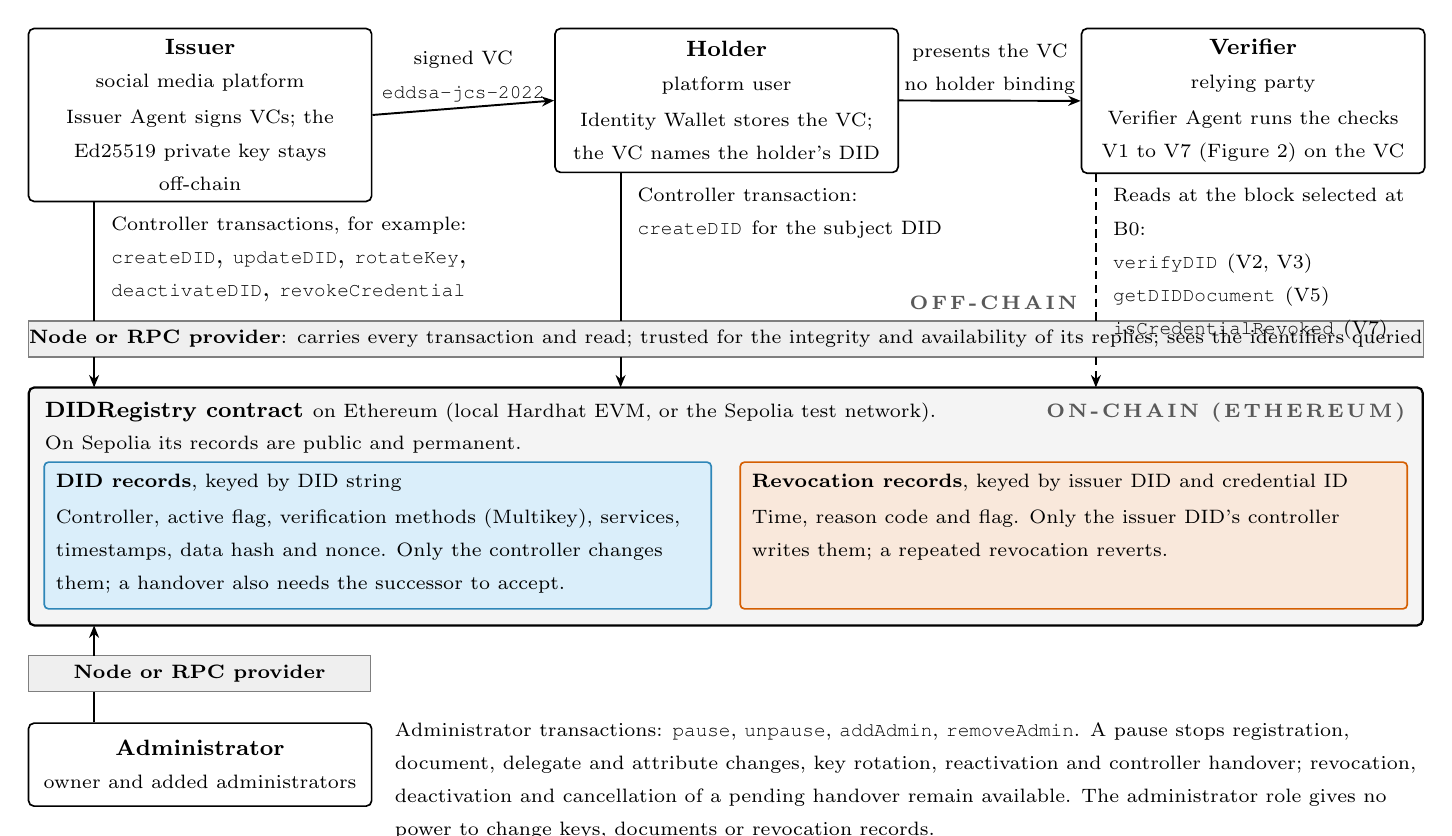
\begin{tikzpicture}[x=1pt,y=1pt,
    actor/.style={draw=black, line width=0.6pt, rounded corners=2pt, fill=white, anchor=north west,
                  minimum width=124pt, minimum height=52pt, text width=116pt, align=flush center, inner sep=4pt},
    call/.style={-{Stealth[length=4.5pt,width=3.6pt]}, line width=0.7pt},
    read/.style={-{Stealth[length=4.5pt,width=3.6pt]}, line width=0.7pt, dash pattern=on 3pt off 2pt},
    callline/.style={line width=0.7pt},
    readline/.style={line width=0.7pt, dash pattern=on 3pt off 2pt},
    note/.style={anchor=north west, inner sep=0pt, align=flush left},
  ]
  \useasboundingbox (0,0) rectangle (504.5,-282);

  % Vertical layout (y downward from 0): actors 0 to -52; arrow notes from -57; node strip \nt to \nb;
  % registry from \rt, height \rh; stub of the node strip \st to \sb under the Administrator arrow (the same height
  % and the same 11 pt gap to the registry as the main strip); administrator box from \at, height 30.
  \def\nt{-106} \def\nb{-119}
  \def\rt{-130} \def\rh{86}
  \def\st{-227} \def\sb{-240}
  \def\at{-251}
  % x positions of the three vertical arrows
  \def\xIss{24} \def\xHol{214.25} \def\xVer{386}

  % Actors (off-chain)
  \node[actor] (I) at (0,0)
    {{\head Issuer}\\{\lab social media platform}\\[1pt]{\lab Issuer Agent signs VCs; the Ed25519 private key stays off-chain}};
  \node[actor] (H) at (190.25,0)
    {{\head Holder}\\{\lab platform user}\\[1pt]{\lab Identity Wallet stores the VC; the VC names the holder's DID}};
  \node[actor] (V) at (380.5,0)
    {{\head Verifier}\\{\lab relying party}\\[1pt]{\lab Verifier Agent runs the checks V1~to~V7 (Figure~2) on the VC}};

  % Horizontal transfers
  \draw[call] (I.east) -- (H.west)
    node[midway, above=1pt, inner sep=1pt, align=flush center] {\lab signed VC\\\fn{eddsa-jcs-2022}};
  \draw[call] (H.east) -- (V.west)
    node[midway, above=1pt, inner sep=1pt, align=flush center] {\lab presents the VC\\\lab no holder binding};

  % Layer label of the actor row: flush right just above the node strip, in the free space left of the dashed read line
  \node[anchor=base east, inner sep=0pt] at (\xVer-6,\nt+4) {\layer{OFF-CHAIN}};

  % Node or RPC provider: every transaction and read passes through it (the arrows break at the strip).
  % Outlines are inset by half their line width, so that the strokes at the canvas edge are not clipped.
  \draw[line width=0.4pt, draw=greyline, fill=nodefill] (0.2,\nt) rectangle (504.3,\nb);
  \node[anchor=center, inner sep=0pt] at (252.25,{(\nt+\nb)/2})
    {\fontsize{7}{8}\selectfont\textbf{Node or RPC provider}: carries every transaction and read; trusted for the integrity and availability of its replies; sees the identifiers queried};

  % Registry (on-chain)
  \draw[line width=0.8pt, rounded corners=2pt, fill=regfill] (0.4,\rt) rectangle (504.1,\rt-\rh);
  \node[anchor=north east, inner sep=0pt] at (498.5,\rt-5.5) {\layer{ON-CHAIN (ETHEREUM)}};
  \node[note, text width=392pt] at (6,\rt-5)
    {{\head DIDRegistry contract} {\lab on Ethereum (local Hardhat EVM, or the Sepolia test network).}\\[-0.5pt]
     {\lab On Sepolia its records are public and permanent.}};
  \draw[line width=0.6pt, draw=skyline, rounded corners=1.5pt, fill=oisky!22] (6,\rt-27) rectangle (247,\rt-80);
  \node[note, text width=233pt] at (10,\rt-31)
    {{\lab\bfseries DID records}{\lab, keyed by DID string}\\[1pt]
     {\lab Controller, active flag, verification methods (Multikey), services, timestamps, data hash and nonce. Only the controller changes them; a handover also needs the successor to accept.}};
  \draw[line width=0.6pt, draw=oiverm, rounded corners=1.5pt, fill=oiverm!14] (257.5,\rt-27) rectangle (498.5,\rt-80);
  \node[note, text width=233pt] at (261.5,\rt-31)
    {{\lab\bfseries Revocation records}{\lab, keyed by issuer DID and credential ID}\\[1pt]
     {\lab Time, reason code and flag. Only the issuer DID's controller writes them; a repeated revocation reverts.}};

  % Issuer controller transactions (solid), through the node strip
  \draw[callline] (\xIss,0 |- I.south) -- (\xIss,\nt);
  \draw[call] (\xIss,\nb) -- (\xIss,\rt);
  \node[note, text width=150pt] at ([yshift=-5pt]\xIss+6,0 |- I.south)
    {{\lab Controller transactions, for example:}\\ \fn{createDID}, \fn{updateDID}, \fn{rotateKey},\\ \fn{deactivateDID}, \fn{revokeCredential}};
  % Holder registers the subject DID (solid)
  \draw[callline] (\xHol,0 |- H.south) -- (\xHol,\nt);
  \draw[call] (\xHol,\nb) -- (\xHol,\rt);
  \node[note, text width=150pt] at ([yshift=-5pt]\xHol+6,0 |- H.south)
    {{\lab Controller transaction:}\\ \fn{createDID} {\lab for the subject DID}};
  % Verifier reads (dashed)
  \draw[readline] (\xVer,0 |- V.south) -- (\xVer,\nt);
  \draw[read] (\xVer,\nb) -- (\xVer,\rt);
  \node[note, text width=112pt] at ([yshift=-5pt]\xVer+6,0 |- V.south)
    {{\lab Reads at the block selected at B0:}\\ \fn{verifyDID} {\lab (V2, V3)}\\ \fn{getDIDDocument} {\lab (V5)}\\ \fn{isCredentialRevoked} {\lab (V7)}};

  % Administrator: its transactions also pass through the node or RPC provider (stub of the strip)
  \node[actor, minimum height=30pt, minimum width=124pt] (A) at (0,\at)
    {{\head Administrator}\\{\lab owner and added administrators}};
  \draw[line width=0.4pt, draw=greyline, fill=nodefill] (0.2,\st) rectangle (124,\sb);
  \node[anchor=center, inner sep=0pt] at (62.1,{(\st+\sb)/2}) {\fontsize{7}{8}\selectfont\textbf{Node or RPC provider}};
  \draw[callline] (\xIss,\at) -- (\xIss,\sb);
  \draw[call] (\xIss,\st) -- (\xIss,\rt-\rh);
  \node[note, text width=372pt] at (132.5,\at)
    {{\lab Administrator transactions: \fn{pause}, \fn{unpause}, \fn{addAdmin}, \fn{removeAdmin}. A pause stops registration, document, delegate and attribute changes, key rotation, reactivation and controller handover; revocation, deactivation and cancellation of a pending handover remain available. The administrator role gives no power to change keys, documents or revocation records.}};
\end{tikzpicture}
\end{document}
